\selectlanguage{italian}

Lo studio delle molecole, ed in particolare delle molecole diatomiche, permette di illustrare due concetti fondamentali nello studio della fisica della materia: la separazione adiabatica del moto elettronico da quello nucleare ed il legame chimico.

\section{Separazione adiabatica}

L'Hamiltoniana per un sistema generico di $ M $ nuclei ed $ N $ elettroni è:
\begin{equation}
	\mathcal{H} = T_n + T_e + V_{ne} + V_{nn} + V_{ee}
	\label{eq:mol-ham-tot}
\end{equation}
Sebbene la funzione d'onda totale del sistema $ \Psi(r,R) $ dipenda dalle coordinate $ r $ di tutti gli elettroni ed $ R $ di tutti i nuclei, è possibile semplificare il problema. Infatti, essendo le masse dei nuclei e quelle degli elettroni diverse di circa tre ordini di grandezza, si può considerare che anche le time-scales dei moti dei nuclei siano tre ordini di grandezza maggiori rispetto a quelle dei moti degli elettroni: c'è dunque un disaccoppiamento dei due moti\footnotemark, in quanto si può assumere che il moto nucleare non induca alcuna transizione sugli stati elettronici (poiché le energie dei moti nucleari sono troppo piccole per colmare i gap energetici tra stati elettronici), da cui il nome di \textit{separazione adiabatica} (o di Born-Oppenheimer).

\footnotetext{In maniera approssimativa, si può dire che gli elettroni percepiscono i nuclei come fermi, mentre i nuclei risentono solo degli effetti medi del moto elettronico.}

\begin{definition}{Fattorizzazione adiabatica}{}
	La funzione d'onda totale del sistema si fattorizza come:
	\begin{equation}
		\Psi(r,R) = \Phi(R) \psi_e(r,R)
	\end{equation}
	dove $ \Phi(R) $ è la \textit{funzione d'onda nucleare} e $ \psi_e(r,R) $ è la \textit{funzione d'onda elettronica}, la quale è soluzione dell'equazione d'onda elettronica:
	\begin{equation}
		[T_e + V_{ne}(r,R) + V_{ee}(r)] \psi_e^{(a)}(r,R) = E_e^{(a)}(R) \psi_e^{(a)}(r,R)
		\label{eq:mol-elc-eq}
	\end{equation}
	con $ (a) $ set di autovalori.
\end{definition}

La funzione d'onda $ \psi_e^{(a)}(r,R) $ descrive un autostato elettronico per una geometria fissata dei nuclei: la dipendenza da $ R $ di $ \psi_e^{(a)}(r,R) $ ed $ E_e^{(a)}(R) $ è puramente parametrica.

\begin{proposition}{Equazione d'onda nucleare}{}
	La funzione d'onda nucleare $ \Phi(R) $ è soluzione dell'equazione d'onda nucleare:
	\begin{equation}
		[T_n + V_\text{ad}^{(a)}(R)] \Phi(R) = E_\text{tot} \Phi(R)
		\label{eq:mol-nucl-eq}
	\end{equation}
	dove il \textit{potenziale adiabatico totale} è:
	\begin{equation}
		V_\text{ad}^{(a)}(R) \equiv E_e^{(a)}(R) + V_{nn}(R)
	\end{equation}

	\tcblower

	\begin{proof}
		Partendo dall'Eq. \ref{eq:mol-ham-tot}:
		\begin{equation*}
			[T_n + T_e + V_{nn} + V_{ne} + V_{ee}] \Phi(R) \psi_e(r,R) = E_\text{tot} \Phi(R) \psi_e(r,R)
		\end{equation*}
		e notando che, essendo $ T_e \sim \lap_r $, si ha $ T_e [\Phi(R) \psi_e(r,R)] = \Phi(R) T_e \psi_e(r,R) $:
		\begin{equation*}
			- \sum_\alpha \frac{\hbar^2}{2M_\alpha} \lap_{R_\alpha} [\Phi(R) \psi_e(r,R)] + \Phi(R) \underbrace{[T_e + V_{nn} + V_{ne}] \psi_e(r,R)}_{\text{equazione elettronica}} + \Phi(R) V_{nn} \psi_e(r,R) = E_\text{tot} \Psi(r,R)
		\end{equation*}
		Il primo termine diventa:
		\begin{equation*}
			\begin{split}
				- \sum_\alpha \frac{\hbar^2}{2m_\alpha} \lap_{R_\alpha} [\Phi(R) \psi_e(r,R)]
				= & - \sum_\alpha \frac{\hbar^2}{2M_\alpha} [\Phi(R) \lap_{R_\alpha} \psi_e(r,R) + 2 \nabla_{R_\alpha} \Phi(R) \cdot \nabla_{R_\alpha} \psi_e(r,R)] \\
				& - \psi_e(r,R) \sum_\alpha \frac{\hbar^2}{2M_\alpha} \lap_{R_\alpha} \Phi(R)
			\end{split}
		\end{equation*}
		I primi due termini (non-adiabatici) possono essere ignorati in approssimazione adiabatica, così da rimanere solo col terzo:
		\begin{equation*}
			\psi_e^{(a)}(r,R) [T_n + E_e^{(a)}(R) + V_{nn}(R)] \Phi(R) = E_\text{tot} \Phi(R) \psi_e^{(a)}(r,R)
		\end{equation*}
		Moltiplicando per $ \psi_e^{(a)}(r,R) $ da sinistra ed integrando su tutte le $ r $ si ottiene infine la tesi.
	\end{proof}
\end{proposition}

L'equazione elettronica presenta, nel caso $ N > 1 $, le stesse complicazioni della trattazione dei MEAs, ed è ugualmente risolvibile col metodo HF (con l'ulteriore complicazione che ora bisogna considerare varie geometrie molecolari date dalle $ R $): una volta selezionato lo stato elettronico $ a $, esso segue adiabaticamente il moto nucleare, non transizionando ad altri stati $ a' \neq a $ (questa è un'approssimazione della realtà). \\
Per quanto riguarda l'equazione nucleare, essa esprime il moto dei nuclei all'interno del potenziale adiabatico totale, composto da un termine Coulombiano repulsivo ed un contributo elettronico attrattivo (è ciò che permette alle molecole di esistere come stati legati). $ V_\text{ad}^{(a)}(R) $, funzione di $ 3M $ variabili, presenta una simmetria roto-traslazionale: ciò suggerisce che esso dipenda dalle distanze relative tra i nuclei atomici. Un esempio di andamento di $ V_\text{ad}^{(a)}(R) $ è riportato in Fig. \ref{ad-pot} (per il ground state di una molecola diatomica): si vede che il potenziale ha un minimo $ R_\text{m} $ finito, attorno al quale avvengono le oscillazioni del moto nucleare a bassa temperatura.

\begin{figure}
	\centering
	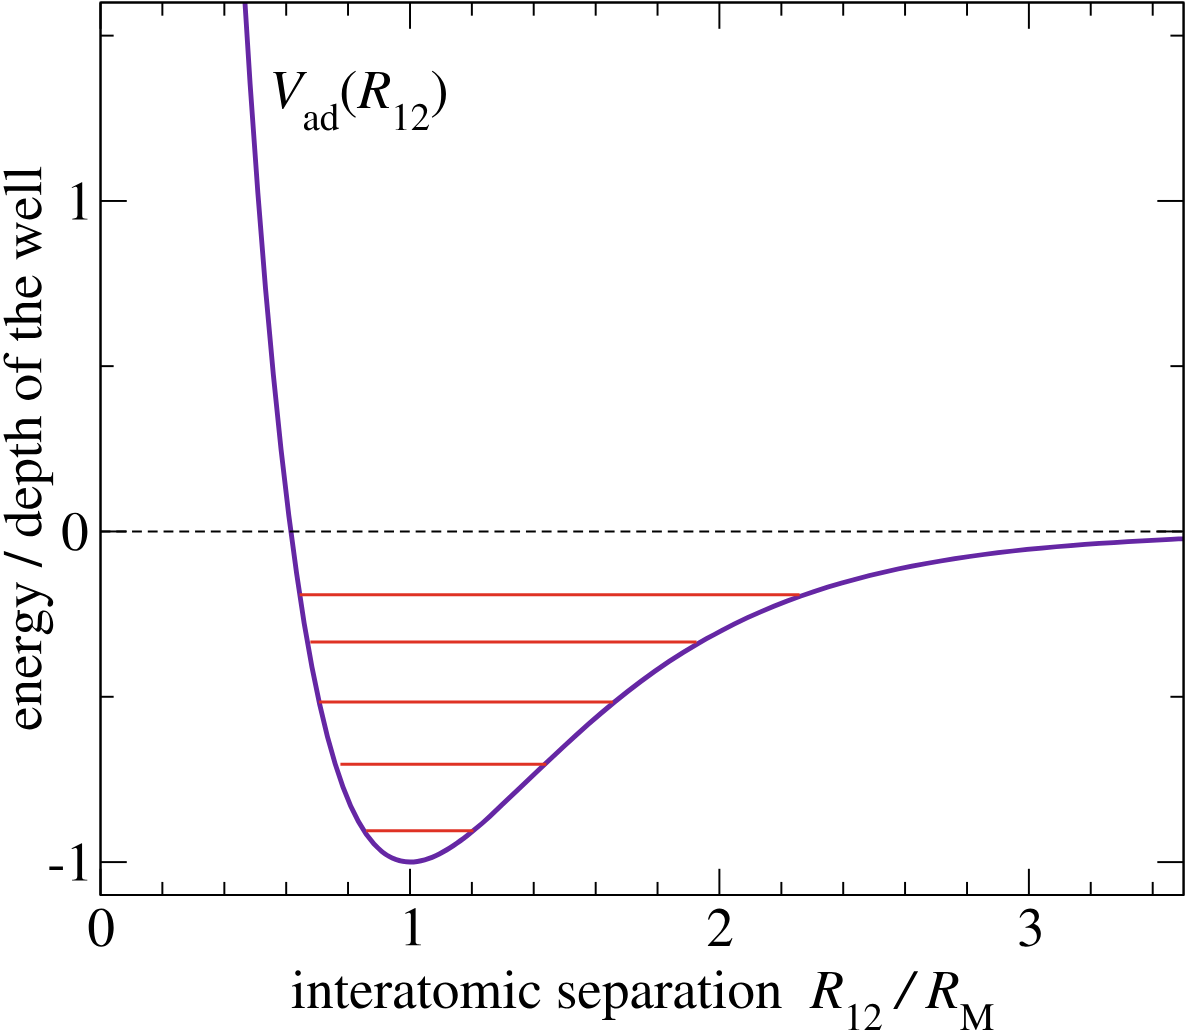
\includegraphics[width = 0.50 \textwidth]{adiabatic-potential.png}
	\caption{Adiabatic potential for a diatomic molecule.}
	\label{ad-pot}
\end{figure}










